\chapter{ART Internals: App Execution}
\label{chapter:art_internals_app_execution}

A running app can be tracked with linux tools that are capable
of showing processes like ``\code{ps}''. To investigate the app execution
we therefore have to open a root shell at the target device
(device should be rooted) with ``\code{adb shell}''
followed by an ``\code{su}'' command after getting the
device prompt (``\code{shell@flounder:/ \$}''). It will then change
to ``\code{root@flounder:/ \#}''. A ``\code{ps}'' command will display
useful information like it's ``USER'', the process id ``PID'',
the process id of its parent ``PPID'' and of course the actual name.
Interesting entries for further inspection are being displayed in
\autoref{tab:ps_entries}.

\begin{table}[htb]
  \caption[Android Processes]{Android processes}
  \label{tab:ps_entries}
  \centering
  \begin{tabular}{l l l l l}
    \toprule
      USER & PID & PPID & ... & NAME \\
    \midrule
      root & 1 & 0 & ... & /init \\
      root & 211 & 1 & ... & zygote64 \\
      root & 212 & 1 & ... & zygote \\
      u0\_a137 & 10072 & 211 & ... & ma.schleemilch.helloandroid \\
      u0\_a35 & 11017 & 212 & ... & com.android.chrome \\
    \bottomrule
  \end{tabular}
\end{table}

The process ``\code{/init}'' is the first process of Android (although
it has a parent with PID ``0'' which is the process scheduler at kernel
level).
Furthermore, every user and system app has either the process
``\code{zygote}'' or ``\code{zygote64}'' as its parent depending
if the app was written for 32 or 64 bit. That makes clear that apps
are forked from the Zygote process that is in turn forked out of
``\code{/init}''. Even more detailed information about processes can be
pulled out of the ``\code{/proc}'' directory. It is an interface to the
kernel and does contain a folder for every process, named after its PID
\parencite{proc}. The most attractive attribute of that folder is
``\code{exe}'' which is a symbolic link to the executable that started
the process. Since apps are a fork of Zygote, they should point
to the same executable, which they do (see \autoref{tab:process_executables}).

\begin{table}[htb]
  \caption[Process Executables]{Process starting executables}
  \label{tab:process_executables}
  \centering
  \begin{tabular}{l l}
    \toprule
    \multicolumn{2}{l}{root@flounder:/ \# ls -la /proc/10072/exe} \\
    ... & exe -> /system/bin/app\_process64\_original\\
    \midrule
    \multicolumn{2}{l}{root@flounder:/ \# ls -la /proc/211/exe} \\
    ... & exe -> /system/bin/app\_process64\_original\\
    \midrule
    \multicolumn{2}{l}{root@flounder:/ \# ls -la /proc/11017/exe} \\
    ... & exe -> /system/bin/app\_process32\\
    \midrule
    \multicolumn{2}{l}{root@flounder:/ \# ls -la /proc/212/exe} \\
    ... & exe -> /system/bin/app\_process32\\
    \bottomrule
  \end{tabular}
\end{table}

An executable named ``\code{app\_process32/64}'' seems like to be the entry-point for apps to be started. The responsible program of that executable
can be found in the Android Open Source Project (AOSP) where
``\code{app\_main.cpp}'' is the name of the source code file that gets
compiled into the 32 or 64 bit version
and can be found at ``\code{/frameworks/base/cmds/app\_process/}''.
However, apps cannot be started directly through that program but
only through Zygote which will fork itself into that new app. Zygote
itself will get started through the ``\code{/init}'' process that starts
native daemons and among other things calls ``\code{app\_process}''
in order to init Zygote.

The best thing to do when analyzing source code is to start at the
``\code{main()}'' method. One of the first things the program does is
creating a new ``\code{AppRuntime runtime}'' object that inherits from the
\code{AndroidRuntime} class but does override a few functions. As parameters it will expect the \code{argv[0]}
which is the program name itself as well as the total length of arguments.
In the end the program transfers the flow control to this object by calling
\code{runtime.start(com.android.internal.os.ZygoteInit, args)}.
``\code{args}'' does contain whether to start the system server and an ABI
list as well as remaining arguments that were not used for the \code{app\_process} program. The runtime \code{start()} method does initialize
a VM and finally does call the main method of the \code{ZygoteInit.java}
program in case of a Zygote start.

\section{Zygote}\label{section:zygote}
\code{ZygoteInit's} main starts with parsing arguments such as if a system
server should get started, the ABI list and the socket name that Zygote will
create. That defined socket (\code{LocalServerSocket sServerSocket}) is a core functionality of Zygote whose purpose
is to listen on that socket and  finally fork Zygote and specialize it afterwards. After registering that socket a preload method loads classes
resources, OpenGL and shared libraries and a explicit garbage collection
\code{gc()} will be performed to clean up after startup. After the optional start of the system server, the program will enter its main loop
\code{runSelectLoop(abiList)}. Garbace collection gets explicity called
after \code{GC\_LOOP\_COUNT} iterations. Right before the loop an array list for file descriptors (\code{ArrayList<FileDescriptor> fds}) as well as for socket connections (\code{ArrayList<ZyogteConnection> peers}) is being
created and \code{fds} gets filled with the server socket file descriptor.
\autoref{zygote_init_loop} displays the logic of the main loop.

\lstinputlisting[language=Java, caption=ZygoteInit main loop, label=zygote_init_loop,firstline=773, lastline=795]{"code/ZygoteInit.java"}

First the file descriptor list is converted to an array and index gets
filled with a readable file descriptor. If that index is zero,
a new \code{ZygoteConnection} is established which is listening
on its defined socket and accepting pending connections.
Afterwards, it gets added to the \code{peer}
and \code{fds} list.
The \code{acceptComandPeer()} method does
call the \code{ZygoteConnection} constructor with \code{sServerSocket.accept()}
as transfer parameter which is an extension to the \code{LocalSocket}
implementation. Its \code{accept()} method accepts a new connection
to the socket and blocks until a new socket arrives.
Therefore the next iteration delivers an index greater than zero so that
the last \code{else} branch of \autoref{zygote_init_loop} is executed within
a \code{ZygoteConnection} object of \code{peers} at that index calls
the \code{runOnce()} method and gets removed out of the array lists afterwards.
Finally the \code{runOnce()} method will call \code{Zygote.forkAndSpecialize()}
that forks a child within an exception is being called to invoke the childs
\code{main()}.
But first the given arguments from the command socket must be parsed with the
aid of an \code{Arguments} class. Attributes that are needed for the later \code{fork()} call are shown in \autoref{tab:argument_class_attributes}.

\begin{table}[htb]
  \caption[Arguments Class Attributes]{Arguments Class Attributes}
  \label{tab:argument_class_attributes}
  \centering
  \begin{tabular}{l l l}
    \toprule
     Given Argument & Attribute & Description \\
     \midrule
     -{}-setuid & int uid & UNIX uid for the child \\
     -{}-setgid & int gid & UNIX gid for the child \\
     -{}-setgroups & int gids[] & additional groups \\
     -{}-enable-debugger & int debugFlags & debug information \\
     -{}-enable-checkjni & int debugFlags & debug information \\
     -{}-enable-assert & int debugFlags & debug information \\
     -{}-enable-safemode & int debugFlags & debug information \\
     -{}-enable-jni-logging & int debugFlags & debug information \\
     -{}-mount-external & int mountExternal & storage to mount \\
     -{}-target-sdk-version & int targetSdkVersion & target version \\
     -{}-classpath & String classpath & absolute classpath \\
     -{}-runtime-init & boolean runtimeInit & new runtime init \\
     -{}-nice-name & String niceName & process renaming \\
     -{}-instruction-set & String instructionSet & instruction set to use \\
     -{}-seinfo & String seInfo & SELinux infos  \\
     -{}-rlimit & ArrayList<int[]> rlimits & resource limitations \\
     -{}-app-data-dir & String appDataDir & data directory \\
      \bottomrule
  \end{tabular}
\end{table}

Then all the defined security policies are being applied. To avoid bad file
descriptor messages after forking a child, a native code has to close them before (\code{sServerSocket} and the local socket \code{mSocket} of the
\code{ZygoteConnection} class whose FDs are written into an \code{fdsToClose}
array).
Now all prerequisites of forking are fulfilled and the static method
\code{forkAndSpecialize} of the \code{Zygote.java} file can be called
(see \autoref{zygote_fork}) returning the new process PID.
\begin{lstlisting}[language=Java, caption=Zygote Fork Call, label=zygote_fork]
pid = Zygote.forkAndSpecialize(parsedArgs.uid, parsedArgs.gid,
            parsedArgs.gids, parsedArgs.debugFlags, rlimits,
            parsedArgs.mountExternal, parsedArgs.seInfo,
            parsedArgs.niceName, fdsToClose,
            parsedArgs.instructionSet,
            parsedArgs.appDataDir);
\end{lstlisting}
\code{Zygote.java} is quite compact since it mainly defines the transition
to native code where the actual forking is being applied. That's why
a native version of the fork and specialize method is defined and executed
which in turn returns the resulting PID after forking
(\code{com\_android\_internal\_os\_Zygote.cpp}).
The native implementation does finally call the effective \code{fork()} method
that copies the actual Linux process. Afterwards, the child is being
specialized (selected by the resulting PID of \code{fork()}).
Transfered FDs are being closed and capability boundaries are applied.
UID and GID are being set (Linux \code{setresgid/setresuid}) and resource limits are added via \code{strlimit(2)}.
If necessary, a native bridge will be initialized and scheduler policies
are being set. SELinux properties are applied and the thread name gets finally
changed to another name than ``app\_process''.

Back in the Java world \code{ZygoteConnection} checks the returned PID and either calls \code{handleChildProc()} in case of the child or
\code{handleParentProc()} in case of the parent (Zygote itself).
These methods are handling the post fork setup. In case of the child, sockets are being closed on Java level and remaining arguments are being evaluated. When forking an app, a class name will be defined at that time. Remaining arguments are copied to \code{mainArgs} and a class loader (\code{ClassLoader cloader}) is being defined before calling \code{invokeStaticMain()} of \code{ZygoteInit} with \code{cloader}, \code{className} and \code{mainArgs} as parameters.

The \code{invokeStaticMain()} loads the corresponding class and furthermore
searches for the main function and finally throwing an
\code{MethodAnd\allowbreak ArgsCaller()} exception which gets caught of the main method of \code{Zygote\allowbreak Init}. Remember that the Zygote itself is ``trapped'' in a loop whereas the child process can escape from by throwing that exception.
So as a result, Zygote will remain in the loop offering a socket to fork
itself again while the child process escapes from that loop and
invoking the main method of the class specified over the socket
connection.
To clearify the program flow, \autoref{fig:zygote_forking} displays
the object and therefore file interaction during the forking process.

\begin{figure}[htb]
  \centering
  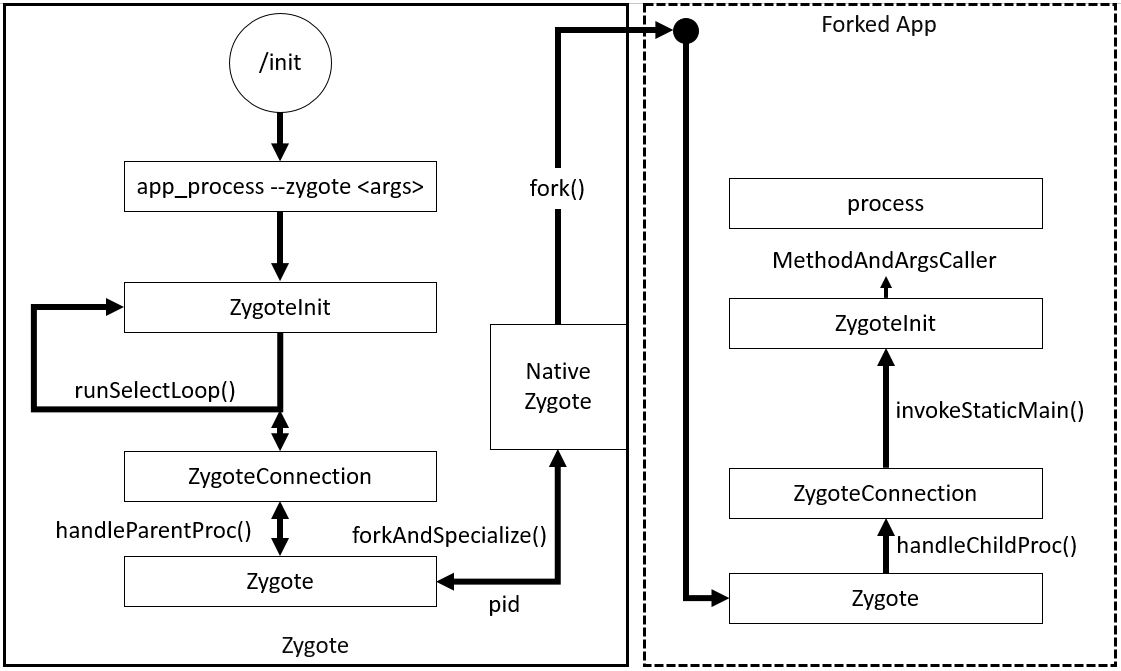
\includegraphics[width={\textwidth}]{figures/zygote_forking}
  \caption[Zygote Forking]{Zygote Forking}
  \label{fig:zygote_forking}
\end{figure}


The current child process state discussed is right after the main loop
breakout of \code{ZygoteInit} induced by the exception. The exception
is actual defined as a class that extends \code{Exception} and implements
\code{Runnable}. Therefore it is viable to call the exception callers
\code{run()} method (see \autoref{child_breakout}).

\lstinputlisting[language=Java, caption=Zygote Child Loop Breakout Exception, label=child_breakout,firstline=697, lastline=699]{"code/ZygoteInit.java"}


\section{Class Loading and Method Invocation}\label{cl_loading}


%ClassLoader??
%Method m.invoke()???


When a user clicks on an app icon, the ``onClick()'' method
of the ``Launcher'' application gets called.




